\chapter{Java para Web}\label{cap:javaParaWeb}
\epigraph{``\textit{Uma longa viagem começa com um único passo}''.}{Lao-Tsé}

\lettrine[lines=4, lhang=0.1, lraise=0, loversize=0.2, findent=0.1em]{\textcolor{corTema}{N}}{ESTE} Capítulo teremos como objetivos entender o funcionamento e a arquitetura de aplicações Web desenvolvidas em Java, entender o funcionamento dos Servlets e dos JSPs e aprender a configurar e a utilizar a \textit{Integrated Development Environment} (IDE) Apache NetBeans para o apoio ao desenvolvimento de aplicações Web em Java.


\section{Introdução}

Para que você seja capaz de construir aplicações Web, primeiramente é preciso conhecer como esse serviço é estruturado. A \textit{World Wide Web} (WWW), ou simplesmente Web, é um serviço executado em diversos computadores interligados em uma rede mundial, sendo que em alguns desses computadores são executados programas chamados de \textbf{servidores}, enquanto na maioria dos outros são executados programas chamados de \textbf{clientes}, que se comunicam com os servidores que, por sua vez, servem recursos para esses clientes. Na Figura~\ref{fig:cap01ClienteServidor} é ilustrado um recorte desta rede mundial.

\FloatBarrier
\begin{figure}[!htbp]
    \centering
    \caption{Recorte da estrutura da WWW}
    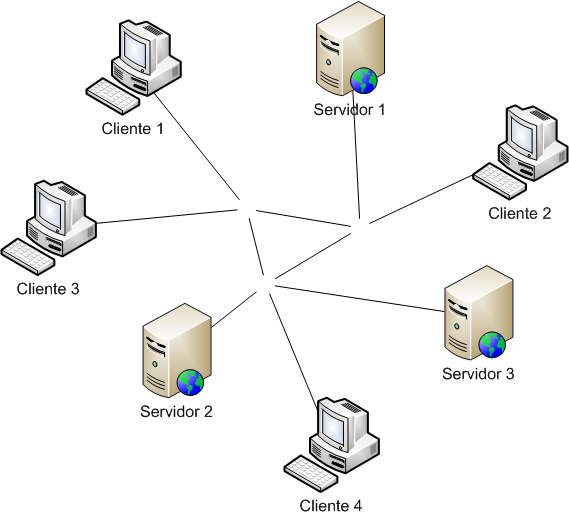
\includegraphics[scale=0.6]{imagens/cap01ClienteServidor}
    \\\textbf{Fonte:} Elaborada pelo autor
    \label{fig:cap01ClienteServidor}
\end{figure}
\FloatBarrier

Perceba que no recorte apresentado na Figura~\ref{fig:cap01ClienteServidor} são mostrados sete computadores, sendo que quatro deles atuam como clientes e os outros três como servidores. É importante entender que o que faz um computador ser cliente ou servidor é o tipo de programa que está sendo usado/executado. No nosso exemplo, as máquinas que atuam como servidores executam um programa denominado Servidor Web, que tem a capacidade de servir (disponibilizar) aos outros computadores da rede, recursos que fazem parte de uma aplicação Web, por exemplo, arquivos \textit{Hypertext Markup Language} (HTML), imagens em diversos formatos, arquivos de estilo, arquivos de \textit{script} etc. Os clientes, por sua vez, são, na maioria das vezes, os conhecidos navegadores Web, ou \textit{browsers}, que usamos no nosso dia a dia para acessar a Web e navegar em diversos \textit{sites}.

Da mesma forma que existem diversos navegadores, existem também alguns Servidores Web, sendo o Apache o mais famoso e o mais utilizado. Como já foi dito, um Servidor Web tem a função de servir recursos requisitados pelos clientes. Vamos aprender como isso funciona. Veja a Figura~\ref{fig:cap01RequestResponse}.

\FloatBarrier
\begin{figure}[!htbp]
    \centering
    \caption{Processo de requisição e resposta (\textit{request}/\textit{response})}
    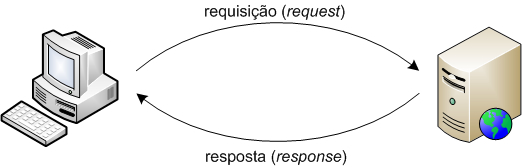
\includegraphics[scale=0.6]{imagens/cap01RequestResponse}
    \\\textbf{Fonte:} Elaborada pelo autor
    \label{fig:cap01RequestResponse}
\end{figure}
\FloatBarrier

Na Figura~\ref{fig:cap01RequestResponse} é mostrado o processo de requisição e resposta. Nesse processo, o cliente à esquerda (navegador), envia uma requisição a um recurso contido no Servidor Web (à direita) através de uma \textit{Uniform Resource Locator} (URL), sendo que nessa requisição, o cliente especifica o protocolo a ser usado, o endereço do servidor e o caminho para o recurso. Assim, uma URL tem a seguinte forma:

\begin{center}
    \textbf{\texttt{protocolo://máquina/caminho\_do\_recurso}}
\end{center}

\begin{itemize}
    
    \item Onde:
    
    \begin{itemize}
    
        \item \textbf{protocolo:} É a parte da URL que diz ao servidor qual o protocolo a ser utilizado. Quando acessamos páginas Web, por padrão, o protocolo utilizado é o \textit{Hypertext Transfer Protocol} (HTTP);
        
        \item \textbf{máquina:} É o nome ou o endereço codificado pelo \textit{Internet Protocol} (IP) da máquina que está executando o Servidor Web;
        
        \item \textbf{caminho\_do\_recurso:} É o caminho completo do recurso desejado que é disponibilizado pelo servidor.
        
    \end{itemize}
    
\end{itemize}

Confuso? Nem tanto. Vamos a um exemplo! Imagine a seguinte situação: Queremos acessar o site do IFSP. Para isso, abra o seu navegador e preencha o campo endereço com \texttt{http://www.ifsp.edu.br/} e tecle \texttt{<ENTER>}. Fazendo isso, o navegador envia uma requisição através de uma URL, usando o protocolo HTTP para a máquina \texttt{www.ifsp.edu.br}, que por sua vez retorna ao navegador uma página HTML que representa aquele endereço. 

Perceba que não especificamos o caminho do recurso! Isso não foi necessário, pois os Servidores Web são normalmente configurados para ter um comportamento padrão para responder às requisições onde só seja especificado o nome da máquina e esse comportamento padrão é direcionar para o recurso \texttt{index.html}, que é um arquivo HTML. Portanto, usar o endereço \texttt{http://www.ifsp.edu.br/} é o mesmo que usar o endereço \texttt{http://www.ifsp.edu.br/index.html}. Faça um teste! Coloque o endereço com o caminho do recurso (\texttt{index.html}) e tecle \texttt{<ENTER>}. O que aconteceu? A mesma página foi exibida não foi? Ótimo!

Vamos fazer mais um teste? Preencha novamente a barra de endereços no seu navegador com o endereço \texttt{https://avatars.githubusercontent.com/u/313050} e tecle \texttt{<ENTER>}. Deve ter aparecido a minha foto, certo? Vamos analisar a URL: usamos o protocolo HTTP, para pedir para o Servidor Web que está executando na máquina \texttt{avatars.githubusercontent.com} o recurso \texttt{313050}, que está armazenado no caminho \texttt{/u/}. Este processo é ilustrado na Figura~\ref{fig:cap01ExemploRequestResponse}.

\FloatBarrier
\begin{figure}[!htbp]
    \centering
    \caption{Exemplo do processo de requisição e resposta a um recurso}
    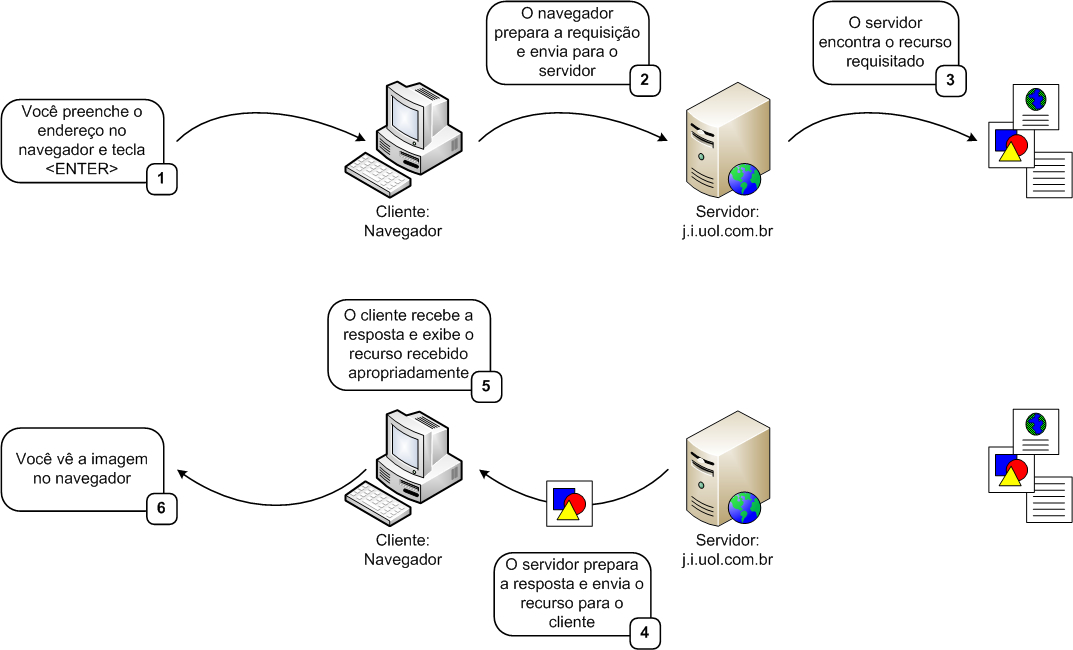
\includegraphics[scale=0.38]{imagens/cap01ExemploRequestResponse}
    \\\textbf{Fonte:} Elaborada pelo autor
    \label{fig:cap01ExemploRequestResponse}
\end{figure}
\FloatBarrier

Perceba que os passos 1, 2 e 3 da Figura~\ref{fig:cap01ExemploRequestResponse} representam o processo de requisição, enquanto os passos 4, 5 e 6 representam o processo de resposta. Note também que ao clicar em qualquer \textit{link}\footnote{O termo \textit{link} será usado para designar os \textit{hyperlinks} dos arquivos HTML} em uma página, todo esse processo é executado pelo navegador.

Muito bem! Agora que você já sabe como funciona o processo de requisição e resposta entre um navegador e um Servidor Web, podemos prosseguir com nossos estudos, agora focando em como a linguagem e a plataforma Java são utilizadas para trabalhar com aplicações Web.


\section{Contêineres de Servlets e Servidores de Aplicações}

Na Seção anterior você aprendeu algumas coisas novas\footnote{Provavelmente você já sabia disso!}, mas onde que a linguagem Java se encaixa nisso tudo? Quando criamos aplicações Web, além de termos páginas com código HTML e outros recursos como imagens, por exemplo, precisamos ter também componentes que processem informações que queremos que nossa aplicação manipule. Imagine que você vai fazer \textit{login} na sua rede social favorita (Facebook, Instagram etc.). Você preenche um campo com seu nome de usuário, sua senha e clica no botão para acessar o sistema e então eu lhe pergunto: O que acontece? Quem que vai validar seu usuário e sua senha? Como você deve saber uma página HTML não consegue fazer isso não é mesmo? Veja a tela de \textit{login} do Facebook na Figura~\ref{fig:cap01LoginFacebook}.

\FloatBarrier
\begin{figure}[!htbp]
    \centering
    \caption{Tela de login da rede social Facebook}
    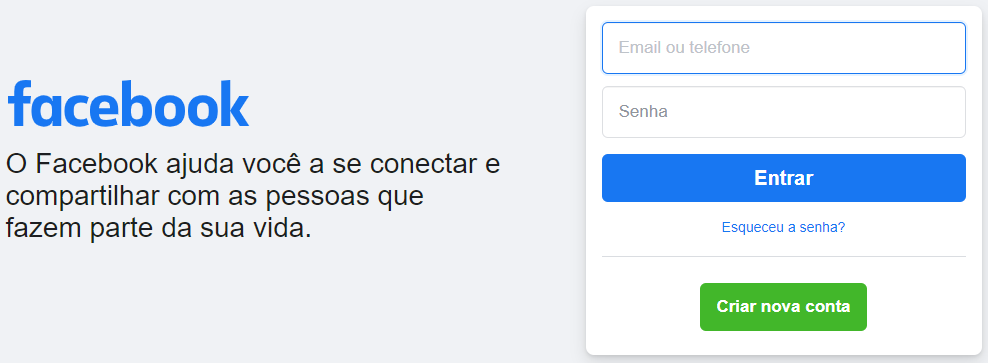
\includegraphics[scale=0.38]{imagens/cap01LoginFacebook}
    \\\textbf{Fonte:} \textit{Print screen} de \url{http://www.facebook.com}, acessado em 21/11/2024
    \label{fig:cap01LoginFacebook}
\end{figure}
\FloatBarrier

O responsável em processar os dados enviados é um componente de software que é executado no servidor em que a aplicação Web está implantada. Se a aplicação é feita em PHP, um script PHP vai fazer essa validação e retornar algum resultado com base no que foi verificado. Se a aplicação for feita em ASP.NET, Node.js etc. acontece o mesmo, ou seja, algum componente vai tratar a requisição -que enviou o usuário e a senha- e vai validá-la. Em Java é a mesma coisa!

Para que possamos utilizar código Java em nossas aplicações Web, recorremos a alguns componentes que podem ser criados dentro delas, sendo que o tipo principal desses componentes é o Servlet. Você se lembra do nosso exemplo do Facebook? Os desenvolvedores do Facebook, se usassem Java, poderiam ter criado um Servlet para receber os dados do formulário de \textit{login}, processá-los e retornar alguma resposta para o cliente, que no caso, normalmente é um navegador.

Muito bem. Sabemos então que se usarmos Java para desenvolver nossas aplicações Web, os componentes que são capazes de processar dados nas nossas aplicações e retornar resultados são os Servlets. Os Servlets são executados e gerenciados pelos Contêineres de Servlets, que funcionam como um Servidor Web simples, mas com alguns ``poderes'' a mais. Esses Contêineres também podem ser componentes de infraestruturas ainda mais robustas, que no caso são os Servidores de Aplicações. Um Servidor de Aplicações é como se fosse um Contêiner de Servlets com anabolizantes, pois além de implementar toda a especificação dos Servlets e as especificações ligadas a eles, esse tipo de servidor também implementa uma série de outras especificações da plataforma Jakarta EE (\textit{Enterprise Edition})\footnote{\url{https://jakarta.ee/}}, antigamente denominada Java EE, que fogem do propósito deste livro.

Da mesma forma que existem navegadores e Servidores Web diferentes, adivinhe só, existem também Servidores de Aplicações e Contêineres de Servlets diferentes! Iremos utilizar a implementação de referência das especificações do Jakarta EE 10, que é feita pelo Servidor de Aplicações Eclipse GlassFish 7.x.x. Trabalharemos especificamente com a versão 7.0.15, pois será a ideal para o que precisaremos fazer e que tem um melhor suporte no NetBeans. Quando estamos no mundo ``Java para Web'', várias dúvidas surgem o tempo todo, visto que existe uma infinidade de termos diferentes e que normalmente causam confusão, além de existir um ecossistema absurdamente vasto. Na próxima seção vamos aprender mais alguns detalhes teóricos e na última seção vamos realizar algumas atividades!


\section{Servlets e JSPs}

Um carro serve para dirigir. Uma televisão para assistir. Uma sandália para andar. Cada um tem suas características e vão evoluindo com o tempo. Há muito tempo, quando foi inventada a televisão, a imagem que era gerada não era muito boa e era em preto e branco. Foram passando os anos e a indústria foi evoluindo o equipamento. Primeiro a imagem melhorou, depois colocaram cores, depois foram criando telas cada vez maiores, mais finas, com maior resolução, inventaram outras formas de emitir imagens, gastar menos energia elétrica e assim por diante. E daí?

Tudo evolui. O que não evolui é descartado e/ou substituído. A primeira especificação dos Servlets foi lançada em 1997 e de lá para cá, a especificação foi evoluindo, permitindo que os Servlets se tornassem componentes mais versáteis e mais fáceis de utilizar. Na versão 7.0.15 do Eclipse GlassFish (perfil \textit{Web}) que implementa as especificações do Jakarta EE 10 (perfil \textit{Web}), é implementada a especificação 6.0 dos Servlets, a especificação 3.1 das JSPs (JavaServer Pages), entre outras.

Já aprendemos que os Servlets são componentes de uma aplicação Web feita em Java e que têm a capacidade de processar dados enviados a eles e gerar respostas. Um Servlet pode gerar como resposta o código HTML de uma página, entretanto essa abordagem era utilizada nas versões mais antigas dos Servlets e é totalmente desencorajada hoje em dia. Como eu disse agora há pouco, tudo evolui. Para que os desenvolvedores não precisassem mais gerar código HTML dentro do código Java de um Servlet, foram inventadas as páginas JSP. Uma página JSP é um arquivo que pode conter –e geralmente contém– código HTML e que pode interagir diretamente com algumas funcionalidades de uma aplicação Web.

A rigor, um JSP é processado pelo Servidor de Aplicações e todo o seu conteúdo é traduzido em um Servlet, que por sua vez é compilado e executado pelo Servidor. Todo esse processo é realizado nos bastidores, então não precisamos nos preocupar com esses detalhes, mas é sempre bom saber um pouquinho como as coisas funcionam não é mesmo?

Por causa desse comportamento de tradução das JSPs para Servlets, nós podemos inserir código Java dentro das JSPs, mas novamente não iremos usar essa abordagem, muito menos irei ensinar como fazer, visto que da mesma forma que gerar HTML dentro de um Servlet manualmente é desencorajado, essa abordagem de inserir código Java dentro das JSPs também não deve ser utilizada. Uma JSP deve ser usada para exibir dados, não para processá-los diretamente usando código Java. Note que não estou dizendo que não iremos manipular dados dentro das JSPs, mas sim que existem formas seguras e corretas para fazer isso. Aprenderemos esses detalhes só no Capítulo~\ref{cap:elTagLibs}, pois até lá, já teremos aprendido outros detalhes que ainda não foram apresentados.


\section{Preparação do Ambiente de Desenvolvimento}

Nesta seção você aprenderá a instalar e configurar a IDE Apache NetBeans e o Servidor de Aplicações Eclipse GlassFish 7.0.15 (perfil \textit{Web}).


\subsection{Apache NetBeans}

Você conhece a linguagem Java, aprendeu a teoria e a prática da programação orientada a objetos e provavelmente usou a IDE Apache NetBeans para escrever seus códigos. Neste livro trabalharemos com a versão 24 desta IDE e nos passos abaixo é explicado como deve ser feito o \textit{download} e a instalação da mesma. Esses passos podem ser pulados caso você já tenha essa versão da ferramenta instalada em seu computador. Além disso, na playlist disponível no \textit{link} \url{https://www.youtube.com/playlist?list=PLqEuQ0dDknqVcfcBHGaYrET7IBfchVS-U} você encontrará tutoriais de preparação de ambientes de desenvolvimento para trabalhar com Java para Web, que serão mantidos atualizados.

\begin{enumerate}

    \item Acesse o endereço: \url{https://dlcdn.apache.org/netbeans/netbeans-installers/24/Apache-NetBeans-24-bin-windows-x64.exe};
    
    \item Ao acessar esse \textit{link}, a versão 24 do Apache NetBeans será baixada;
    
    \item Baixou? Execute o instalador. As versões atuais dos instaladores NetBeans farão a instalação completa da IDE. Basta seguir o assistente, escolher o JDK instalado (recomendo o 17 ou o 21) e aguardar o fim da instalação.
    
\end{enumerate}

Com o NetBeans instalado, abra-o. Caso o esteja executando pela primeira vez, uma página de boas-vindas será exibida. Você pode fechá-la se quiser, além de marcar para que não seja exibida novamente. Antes de criarmos o nosso primeiro projeto Java Web, precisamos baixar, instalar e configurar o Servidor de Aplicações Eclipse GlassFish.


\subsection{Eclipse GlassFish}

Como já dito, iremos instalar a versão 7.0.15 do Eclipse GlassFish. Iremos realizar o download e a instalação dentro do NetBeans 24. Com o NetBeans aberto, do lado esquerdo, clique na aba \textit{Services}. Nessa aba, há um nó chamado \destaque{\textit{Servers}}. Clique com o botão direito do mouse nele e escolha \destaque{\textit{Add Server...}}. Veja a Figura~\ref{fig:cap01Servers}.

\FloatBarrier
\begin{figure}[!htbp]
    \centering
    \caption{Registrando um servidor no NetBeans}
    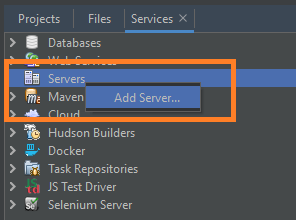
\includegraphics[scale=0.7]{imagens/cap01Servers}
    \\\textbf{Fonte:} Elaborada pelo autor
    \label{fig:cap01Servers}
\end{figure}
\FloatBarrier

Ao clicar em \destaque{\textit{Add Server...}} o assistente para registrar o servidor no NetBeans aparecerá. No primeiro passo, mostrado na Figura~\ref{fig:cap01AddServerP01}, na lista de servidores suportados, escolha \destaque{\textit{GlassFish Server}}. Na caixa de texto \destaque{\textit{Name:}} edite o nome da instância do servidor. No meu caso, adicionei a versão do mesmo, ficando ``GlassFish Server 7.0.15''. Ao fazer isso, clique em \destaque{\textit{Next >}}.

\FloatBarrier
\begin{figure}[!htbp]
    \centering
    \caption{Registrando um servidor no NetBeans - Passo 1}
    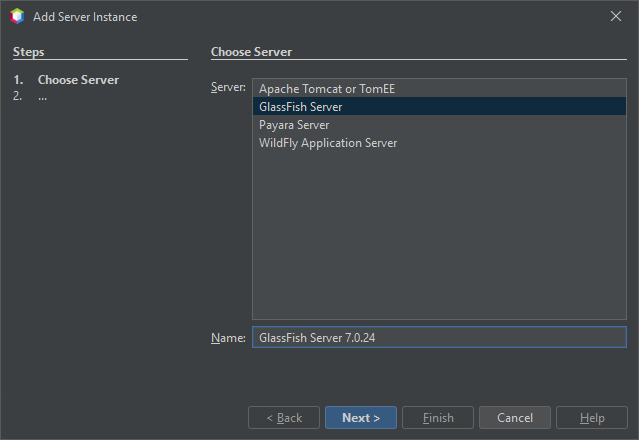
\includegraphics[scale=0.7]{imagens/cap01AddServerInstanceP01}
    \\\textbf{Fonte:} Elaborada pelo autor
    \label{fig:cap01AddServerP01}
\end{figure}
\FloatBarrier

O segundo passo do assistente precisamos definir onde os arquivos do servidor ficarão, como apresentado na Figura~\ref{fig:cap01AddServerP02}. Nesse passo, clique no botão \destaque{\textit{Browse...}} e defina onde a instalação ficará. No meu caso, escolhi a pasta \texttt{glassfish7015} dentro da pasta do meu usuário. Recomendo que você faça o mesmo. Deixa a opção \destaque{\textit{Local Domain}} selecionada, escolha a versão do servidor para download (GlassFish Server 7.0.15), marque a opção ``\textit{I have read...}'' e clique em \destaque{\textit{Download Now}}. Ao finalizar o download, uma mensagem logo abaixo do assistente indicará que foi encontrada uma instalação do servidor no local escolhido, então basta clicar em \destaque{\textit{Next >}} para realizarmos o terceiro e último passo do assistente.

\FloatBarrier
\begin{figure}[!htbp]
    \centering
    \caption{Registrando um servidor no NetBeans - Passo 2}
    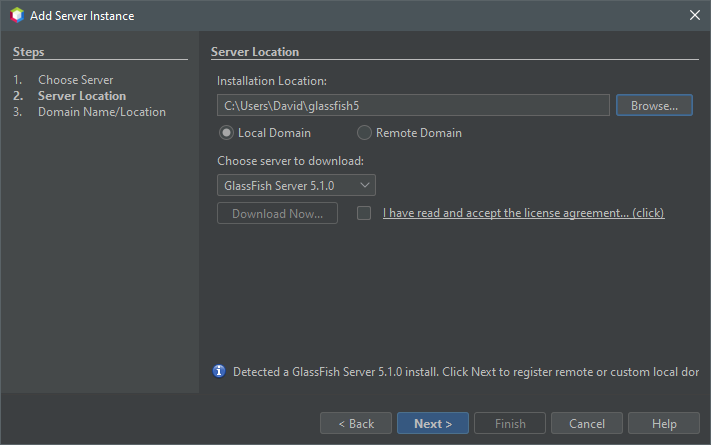
\includegraphics[scale=0.7]{imagens/cap01AddServerInstanceP02}
    \\\textbf{Fonte:} Elaborada pelo autor
    \label{fig:cap01AddServerP02}
\end{figure}
\FloatBarrier

Nesse passo, faremos a última configuração necessária, que consiste apenas em definir o nome do usuário administrador do servidor. Na Figura~\ref{fig:cap01AddServerP03} isso pode ser visto na caixa de texto \destaque{\textit{User Name:}} que está preenchida com ``admin''. Ao preencher o nome de usuário, clique em \destaque{\textit{Finish}}.

\FloatBarrier
\begin{figure}[!htbp]
    \centering
    \caption{Registrando um servidor no NetBeans - Passo 3}
    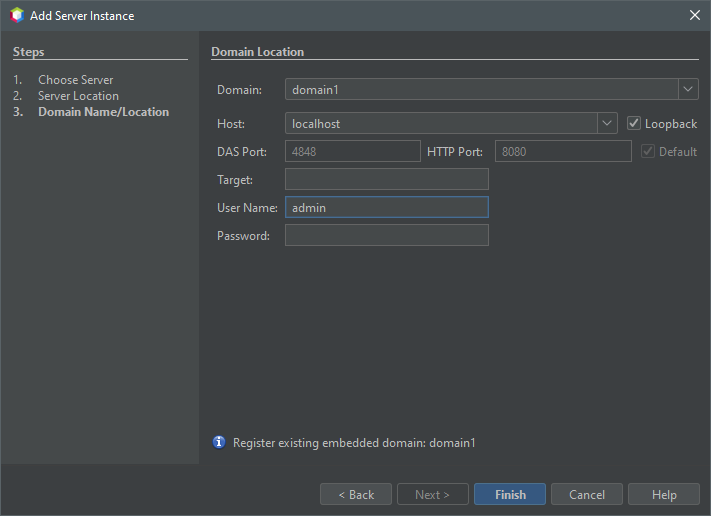
\includegraphics[scale=0.7]{imagens/cap01AddServerInstanceP03}
    \\\textbf{Fonte:} Elaborada pelo autor
    \label{fig:cap01AddServerP03}
\end{figure}
\FloatBarrier

Ao fazer isso, o GlassFish estará quase pronto para ser utilizado. A última coisa que precisaremos fazer é copiar o \textit{Driver Java Database Conectivity} (JDBC) do Sistema Gerenciador de Banco de Dados (SGBD) MariaDB/MySQL que usaremos nos próximos Capítulos deste livro.

Para isso, baixe o arquivo acessível através do \textit{link} \url{https://repo1.maven.org/maven2/org/mariadb/jdbc/mariadb-java-client/3.5.0/mariadb-java-client-3.5.0.jar} e, ao terminar de baixar, copie-o para o diretório \texttt{C:\textbackslash Users\textbackslash SeuUsuario\textbackslash glassfish7015\\\textbackslash glassfish\textbackslash domains\textbackslash domain1\textbackslash lib\textbackslash}. Agora sim, tudo pronto!

Caso haja alguma dúvida, visite o \textit{link} mencionado que contém uma playlist de tutoriais para a configuração de ambientes de desenvolvimento.


\subsection{Primeiro Projeto Java para Web}\label{subsec:primeiroProjeto}

Agora que temos tudo configurado, iremos criar nosso primeiro projeto Java para Web! Siga os passos abaixo:

\begin{itemize}

    \item \textbf{Passo 1:} Clique no menu \destaque{\textit{File}} e depois em  \destaque{\textit{New Project...}}. Fazendo isso, o assistente para criação de projetos será aberto. Na lista de categorias, expanda o item  \destaque{\textit{Java with Ant}} e escolha  \destaque{\textit{Java Web}}. Na lista de tipos de projeto, escolha  \destaque{\textit{Web Application}} e clique no botão  \destaque{\textit{Next >}};
    
    \item \textbf{Passo 2:} Preencha o campo \destaque{\textit{Project Name:}} com ``OlaMundoWeb'' (sem acentos, sem as aspas e tudo junto). Em \destaque{\textit{Project Location:}}, defina o diretório onde o projeto será salvo. Deixe a opção \destaque{\textit{Use Dedicated Folder for Storing Libraries}} marcada e clique no botão \destaque{\textit{Next >}};
    
    \item \textbf{Passo 3:} Na opção \destaque{\textit{Server:}} escolha o ``GlassFish Server 7.0.15'', ou a opção com o nome que você definiu ao registrar o GlassFish. Em \destaque{\textit{Java EE Version:}} escolha ``Jakarta EE 10 Web''. Em \destaque{\textit{Context Path:}} deixe o valor padrão (/OlaMundoWeb), que é o mesmo nome que demos ao nosso projeto. Clique em \destaque{\textit{Next >}};
    
    \item \textbf{Passo 4:} No último passo, o assistente perguntará quais \textit{frameworks} nós queremos inserir no nosso projeto. Nós não vamos usar nenhum, então basta clicar em \destaque{\textit{Finish}}. Fazendo isso, o novo projeto será criado e será aberto no NetBeans, sendo que por padrão será criado um arquivo HTML (\texttt{index.html}) que será a página inicial da nossa aplicação.
    
\end{itemize}

\begin{saibaMais}
    Existem diversas definições para \textit{framework}, sendo que, informalmente, podemos definí-los como um conjunto de classes que incorporam uma abstração que tem como objetivo de solucionar problemas de um tipo ou domínio específico.
\end{saibaMais}

Muito bem, criamos nosso primeiro projeto. Vamos executá-lo para ver o que acontece? Na barra de ferramentas do NetBeans tem um botão com uma seta verde, igual a um botão de ``\textit{play}'' de um reprodutor de mídias. Quando você clicar nesse botão, você vai ver que várias mensagens começarão a aparecer na janela de saída do NetBeans. Essas mensagens irão mostrar para nós o que está acontecendo no momento, como a inicialização do GlassFish (caso não esteja iniciado) etc. O que está esperando? Clique lá no ``\textit{play}''. Assim que tudo estiver pronto, será aberta uma janela do seu navegador, onde será mostrado o conteúdo do \texttt{index.html}, que no nosso caso será uma página com ``TODO write content'' escrito.

Muito bem! Temos nossa primeira aplicação rodando no GlassFish! Fácil não é mesmo? Por enquanto não vamos nos preocupar com a estrutura do projeto, iremos aprender os detalhes aos poucos. Vamos colocar um pouco de código HTML no nosso \texttt{index.html}? Ele deve estar aberto no NetBeans. Se não estiver, procure o arquivo \texttt{index.html} na pasta \destaque{\textit{Web Pages}} do seu projeto e clique duas vezes no arquivo para abri-lo no editor. Vamos mudar o título, escrevendo ``Meu Primeiro Projeto Java para Web'' no lugar de ``TODO supply a title'' e dentro da \textit{tag} \inlineHTMLCode{<body>} do arquivo, inserir um \textit{heading} \inlineHTMLCode{<h1>} e um parágrafo com um \textit{link} para o site do IFSP. Veja na Listagem~\thechapter.\ref{listagem:projetos/capitulo01/OlaMundoWeb/web/index.html} como deve ficar seu código.

\htmlCode{Arquivo \texttt{index.html}}{projetos/capitulo01/OlaMundoWeb/web/index.html}

Salve o arquivo depois de editá-lo. Se o navegador ainda estiver aberto no \texttt{index.html}, volte a ele e aperte a tecla \texttt{<F5>} do seu teclado para mandar o navegador atualizar a página. Se não estiver, dê o ``\textit{play}'' no projeto de novo. Você vai ver que a página vai exibir as alterações que fizemos. Teste o \textit{link} para ver se está funcionando. A página deve ter ficado como mostrada na Figura~\ref{fig:cap01OlaMundoIndex}.

\FloatBarrier
\begin{figure}[!htbp]
    \centering
    \caption{Arquivo \texttt{index.html} em exibição}
    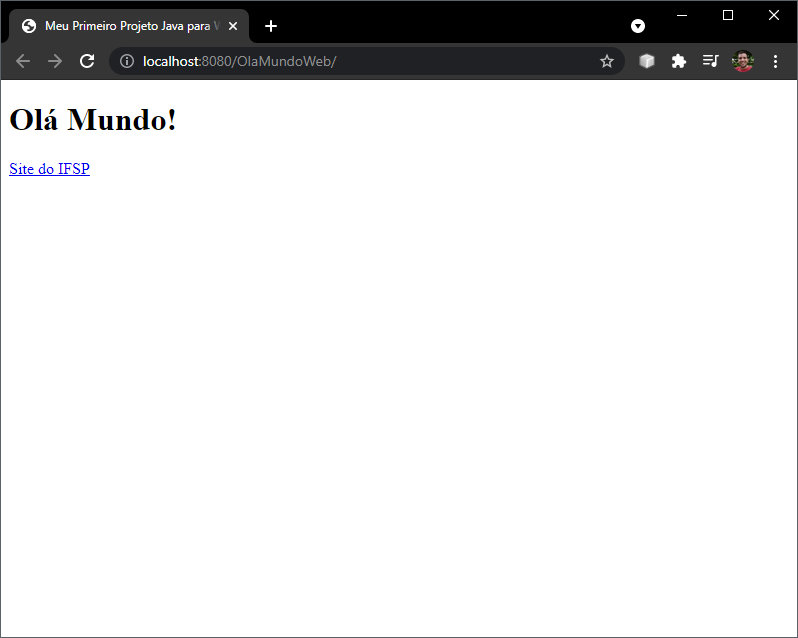
\includegraphics[scale=0.7]{imagens/cap01OlaMundoIndex}
    \\\textbf{Fonte:} Elaborada pelo autor
    \label{fig:cap01OlaMundoIndex}
\end{figure}
\FloatBarrier

Poderíamos ter usado um arquivo \textit{JavaServer Pages} (JSP) ao invés de usar um arquivo HTML, permitindo a existência de outros tipos de estruturas que vamos aprender no decorrer do livro, mas por enquanto vamos manter o HTML. Vamos testar os Servlets agora? Como primeiro exemplo, nós vamos criar um Servlet manualmente, enquanto os outros que vamos desenvolver durante o nosso curso serão feitos usando um assistente do NetBeans, mas essa forma fácil nós só vamos aprender a partir do Capítulo~\ref{cap:processamentoFormularios}.

Aprenderemos como criar manualmente um Servlet, para que possamos aprender alguns detalhes importantes sobre o funcionamento de aplicações Web feitas em Java. Siga os passos abaixo:

\begin{itemize}
    
    \item \textbf{Passo 1:} Na árvore que representa a estrutura do projeto, procure pela pasta \destaque{\textit{Source Packages}} e expanda-a (clique no sinal de ``+'' à esquerda). Dentro dela haverá um pacote com o ícone cinza chamado \destaque{\textit{<default package>}}. Como vocês devem saber, é desencorajado que se trabalhe com pacotes padrão em Java, então vamos criar um pacote. Clique com o botão direito na pasta \destaque{\textit{Source Packages}} e escolha \destaque{\textit{New}}, procure pela opção \destaque{\textit{Java Package...}} e clique nela. Se esta opção não estiver sendo exibida, clique na opção \destaque{\textit{Other...}} (no final da lista), escolha \destaque{\textit{Source Packages}} nas categorias, e \destaque{\textit{Java `Package}} nos tipos de arquivos e clique em \destaque{\textit{Next >}}. Preencha o campo \destaque{\textit{Package Name:}} com ``olamundoweb'' (sem as aspas) e clique em \destaque{\textit{Finish}}. O pacote será criado;
        
    \item \textbf{Passo 2:} Repita o Passo 1, só que agora clicando com o botão direito no pacote que você criou e crie um pacote chamado ``servlets'' (sem as aspas). O nome do pacote deverá ser preenchido com ``olamundoweb.servlets''. Seu projeto agora terá um pacote chamado ``olamundoweb.servlets''. O resultado desses dois primeiros passos podem ser vistos na Figura~\ref{fig:cap01CriacaoPacote};
    
    \FloatBarrier
    \begin{figure}[!htbp]
        \centering
        \caption{Criação do pacote \texttt{olamundoweb.servlets}}
        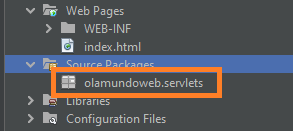
\includegraphics[scale=0.9]{imagens/cap01CriacaoPacote}
        \\\textbf{Fonte:} Elaborada pelo autor
        \label{fig:cap01CriacaoPacote}
    \end{figure}
    \FloatBarrier
            
    \item \textbf{Passo 3:} Clique com o botão direito no pacote  \destaque{\texttt{olamundoweb.servlets}}, escolha \destaque{\textit{New}} e clique na opção \destaque{\textit{Java Class...}}. Novamente, se não a encontrar, clique em \destaque{\textit{Other...}} e procure por \destaque{\textit{Java Class...}} (está na categoria ``Java'') e clique em \destaque{\textit{Next >}}. Preencha o campo \destaque{\textit{Class Name:}} com ``OlaServlet'' (sem as aspas) e clique em \destaque{\textit{Finish}}. A classe será criada dentro do pacote especificado e será aberta no editor. Você vai ter algo como apresentado na Listagem~\thechapter.\ref{listagem:projetos/capitulo01/parciais/OlaServlet.java} (sem os comentários);
    
    \javaCode{olamundoweb/servlets/OlaServlet.java}{projetos/capitulo01/parciais/OlaServlet.java}
    
    \item \textbf{Passo 4:} Para que uma classe seja um Servlet, precisamos estender a classe \texttt{HttpServlet}, que está contida no pacote \texttt{jakarta.servlet.http}\footnote{O Jakarta EE 10 usa o novo \textit{namespace} do Java EE, onde o pacote base é o \texttt{jakarta}. Antes da versão 9 o namespace base era \texttt{javax}.} e então implementar os métodos HTTP que queremos que nosso Servlet trate. Não se preocupe, ainda vamos aprender sobre os métodos HTTP, então o mais importante a saber, por enquanto, é que os métodos HTTP mais usados são o \texttt{GET} (\inlineJavaCode{doGet(...)} de \texttt{HttpServlet}) e o  \texttt{POST} (\inlineJavaCode{doPost(...)} de  \texttt{HttpServlet}). Então teremos que sobrescrever cada um desses métodos e ainda criaremos um terceiro que será invocado a partir dos outros dois. Confuso? Vamos ver como o código ficaria. Leia os comentários e copie o código da Listagem~\thechapter.\ref{listagem:projetos/capitulo01/OlaMundoWeb/src/java/olamundoweb/servlets/OlaServlet.java} para o seu editor.
    
\end{itemize}

\FloatBarrier
\javaCode{olamundoweb/servlets/OlaServlet.java}{projetos/capitulo01/OlaMundoWeb/src/java/olamundoweb/servlets/OlaServlet.java}
\FloatBarrier
    
Até agora criamos uma classe chamada \texttt{OlaServlet}, que estende a classe \texttt{HttpServlet}. Sobrescrevemos os métodos \inlineJavaCode{doGet(...)} e \inlineJavaCode{doPost(...)} herdados de \texttt{HttpServlet} que tratam respectivamente os métodos \texttt{GET} e \texttt{POST} do protocolo HTTP e criamos um terceiro método, chamado \inlineJavaCode{processRequest(...)}, que tem a mesma assinatura dos métodos \inlineJavaCode{doGet(...)} e \inlineJavaCode{doPost(...)} e que é invocado dentro deles. É no \texttt{processRequest} que iremos colocar o código que queremos executar, sendo que no nosso exemplo, estamos mandando imprimir na saída duas Strings: ``Olá Mundo!'' e ``Meu Primeiro Servlet!''. Ou seja, se chamarmos o Servlet usando o método \texttt{GET}, o método \inlineJavaCode{doGet(...)} será invocado e passará o controle para o método \inlineJavaCode{processRequest(...)} que irá imprimir as mensagens na saída. O mesmo acontece para o método \texttt{POST}.

Muito bem, você tem um Servlet totalmente funcional, mas ai você se pergunta: ``Como vou chamar esse Servlet através do navegador?''. Então eu respondo: no código completo, você percebeu que há uma anotação chamada \inlineJavaCode{@WebServlet}? É essa anotação que vai fornecer essa informação\footnote{Antigamente precisávamos fazer o mapemanto em um arquivo \textit{Extensible Markup Language} (XML) (\url{http://pt.wikipedia.org/wiki/XML}) chamado de Descritor de Implantação (DI, em inglês \textit{Deployment Descriptor}), representado pelo arquivo \texttt{web.xml}, o que atualmente, com as versõs mais novas do Jakarta/Java EE, não é mais necessário para algumas situações.}, expecificamente no parâmetro \texttt{urlPatterns}. Perceba que configuramos esse parâmetro com um array de Strings com um elemento: ``/ola''. Com isso, podemos agora acessar o \texttt{OlaServlet} a partir de uma URL, que no nosso caso é ``\url{http://localhost:8080/OlaMundoWeb/ola}'', ou seja, usamos o protocolo HTTP, para a máquina \texttt{localhost} (que é o endereço da nossa máquina), na porta 8080 (que é a porta que o GlassFish ouve por padrão), para acessar a aplicação chamada \texttt{OlaMundoWeb} (isso vem do contexto que criamos no Passo 3 da Subseção~\ref{subsec:primeiroProjeto}, volte lá para dar uma olhadinha), para por fim acessar o recurso mapeado sob o nome de ``ola'' que no caso é o nosso Servlet. 

Sei que pode parecer um pouco confuso no começo, mas logo você vai pegar o jeito da coisa. Dê um ``play'' no projeto de novo. O navegador vai abrir no endereço da aplicação novamente. Insira o ``ola'' (sem as aspas) no final da URL e tecle \texttt{<ENTER>}. O que aconteceu? Apareceu uma página em branco não foi? É claro, afinal, nosso Servlet não gera HTML, mas apenas imprime duas mensagens na saída padrão não é mesmo? Mas como podemos ver essas mensagens? Volte no NetBeans e procure, logo abaixo, uma aba chamada \destaque{\textit{Output}}. Ela provavelmente vai estar selecionada. Dentro dela devem haver outras três abas: \destaque{\textit{OlaMundoWeb (run)}} que deve estar selecionada e que é usada para mostrar o processo de construção do projeto da nossa aplicação, \destaque{\textit{Java DB Database Process}}, que exibe o \textit{status} do Java DB e, por fim, \destaque{\textit{GlassFish Server 7.0.15}}, que exibe a saída padrão do GlassFish. Clique nessa última aba e veja o que está escrito lá embaixo: as duas mensagens que enviamos para a saída padrão através do método \inlineJavaCode{System.out.println(...)} dentro do Servlet, sendo que o fim de cada linha conterá os caracteres \texttt{|\#]}\footnote{Esse sufixo é inserido automaticamente pelo servidor.}! Veja o resultado na Figura~\ref{fig:cap01SaidaGlassFish}. Volte ao navegador e tecle \texttt{<ENTER>} novamente no endereço do Servlet. Volte no NetBeans. Mais duas mensagens! Fácil não é mesmo?

\FloatBarrier
\begin{figure}[!htbp]
    \centering
    \caption{Saída do GlassFish 7.0.15}
    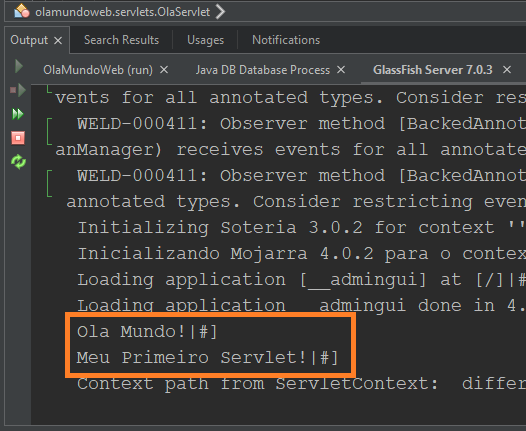
\includegraphics[scale=0.9]{imagens/cap01SaidaGlassFish}
    \\\textbf{Fonte:} Elaborada pelo autor
    \label{fig:cap01SaidaGlassFish}
\end{figure}
\FloatBarrier
    
Por mais que nosso exemplo não tenha nenhuma utilidade aparente, ele foi importante para nós entendermos o funcionamento básico de uma aplicação Web feita em Java. Nos próximos Capítulos vamos colocar o que aprendemos em prática, além de aprender várias outras coisas com o objetivo de criarmos um sistema de cadastro na forma de uma aplicação Web. Não se esqueça de praticar o que aprendemos até agora. 


\section{Resumo}

Neste Capítulo aprendemos o que é e como funciona uma aplicação Web em Java. Aprendemos a criar nosso primeiro projeto e alguns detalhes sobre a tecnologia que estamos utilizando. Executamos nossa aplicação e fizemos algumas modificações nela para vermos o que estava sendo feito. Criamos também –de forma manual– um Servlet, que como aprendemos é um dos componentes principais de uma aplicação Web em Java.


\section{Exercícios}

\begin{exercicioSemArquivo}{}{}{}
    O que é um Servidor Web?
\end{exercicioSemArquivo}

\begin{exercicioSemArquivo}{}{}{}
    Como são chamados os clientes que utilizamos para acessar aplicações servidas por um Servidor Web? Cite alguns exemplos.
\end{exercicioSemArquivo}

\begin{exercicioSemArquivo}{}{}{}
    Diferencie um Servidor Web de um Contêiner de Servlets.
\end{exercicioSemArquivo}


\section{Projetos}

\begin{projetoSemArquivo}{}{}{}
    Crie um novo projeto Java Web no NetBeans, com o nome de ``MinhaPagina'', edite o \texttt{index.html} de modo a exibir seus dados pessoais, seus interesses etc. Tente inserir uma imagem também. Dica: a imagem deve estar dentro do projeto do NetBeans. Pense se você entende o motivo pelo qual o arquivo \texttt{index.html} é mostrado por padrão quando você acessa sua página através da URL \url{HTTP://localhost:8080/MinhaPagina}.
\end{projetoSemArquivo}

\begin{projetoSemArquivo}{}{}{}
    Crie um novo projeto Java Web no NetBeans, com o nome de ``Contador''. Nesse projeto você deve criar um Servlet manualmente e dentro do método \inlineJavaCode{processRequest(...)} use uma estrutura de repetição para direcionar para a saída padrão os números de 1 a 30.
\end{projetoSemArquivo}

\begin{projetoSemArquivo}{}{}{}
    Crie um novo projeto Java Web no NetBeans, com o nome de ``Fibonacci''. Nesse projeto, você deve criar um Servlet manualmente e dentro do método \inlineJavaCode{processRequest(...)} use uma estrutura de repetição para exibir os 30 primeiros termos da série de Fibonacci. Crie um método chamado \texttt{fibonacci} dentro do seu Servlet, sendo que este método deve receber como parâmetro um inteiro e retornar um inteiro. O inteiro que é recebido como parâmetro é o número do termo desejado, enquanto o inteiro que é retornado é o termo correspondente ao parâmetro que foi recebido. A série de Fibonacci é formada inicialmente pelos números 1 e 1, sendo que os próximos números da série são gerados a partir da soma dos dois números anteriores. Os sete primeiros termos da série de Fibonacci são $1, 1, 2, 3, 5, 8, 13$, onde: $2 = 1 + 1, 3 = 1 + 2, 5 = 2 + 3, 8 = 3 + 5, 13 = 5 + 8$.
    
    Exemplos de chamadas da função fibonacci:
    \begin{itemize}
        \item \texttt{fibonacci(2)}: retorna 1
        \item \texttt{fibonacci(5)}: retorna 5
        \item \texttt{fibonacci(7)}: retorna 13
    \end{itemize}
    
\end{projetoSemArquivo}